%Chapter 2

\chapter{Apprentissage profond}

\section{Introduction}

	Quelles sont les limites de l'intelligence des ordinateurs? C'est une question toujours ouverte, même en étant l'une des toutes premières à être posées depuis l'invention des ordinateurs. Dans ce chapitre nous allons présenter l'une des techniques utilisées en intelligence artificielle à savoir l'apprentissage automatique qui permet de doter l'ordinateur d'une capacité d'apprendre et de s'adapter en fonction de la tâche qu'il doit accomplir.
	
	Nous aborderons ensuite l'une des techniques les plus récentes de l'apprentissage automatique qui est l'apprentissage profond (Deep Learning), elle propose une nouvelle approche plus approfondie et plus ressemblante au comportement du cerveau.


\section{Apprentissage automatique}

	On peut trouver dans un dictionnaire que l'apprentissage est: "La capacité d'acquérir et d'appliquer les connaissances". C'est une notion que l'être humain développe depuis son enfance. Question: et si les ordinateurs arriveraient à développer la capacité d'apprendre?

	La tâche de l'apprentissage automatique est de concevoir un algorithme d'apprentissage fiable pouvant être utilisé pour résoudre différents problèmes et être appliqué dans différents domaines. Son utilisation pourrait couvrir plusieurs tâches très distinctes telles que la prévision du marché boursier, la découverte de caractéristiques et motifs dans les données scientifiques ou même la reconnaissance d'objets dans les images.

	En effet, à travers l'exploration du processus d'apprentissage du cerveau, les scientifiques ont fait l'hypothèse qu'il pourrait y avoir un algorithme d'apprentissage unique utilisé pour une variété de tâches. Cet algorithme unique pourrait donc à lui tout seul s'adapter à tous les problèmes qu'il rencontre. 

	Une expérience [figure 3.1] a été conçue en neuroscience au Département du MIT de Brain and Cognitive Sciences [Roe et al. 92], où ils ont coupé le lien entre l'oreille et le cortex auditif de furets, et lui ont relié les nerfs optiques (Le cortex auditif étant la partie du cerveau responsable des processus qui traitent l'information auditive capturé par l'oreille). Ils ont découvert que le cortex auditif a pu apprendre à traiter les données optiques. En d'autres termes, la partie du cerveau qui une fois a appris à entendre, maintenant apprend à voir.

\begin{figure}[H]
	\centering
		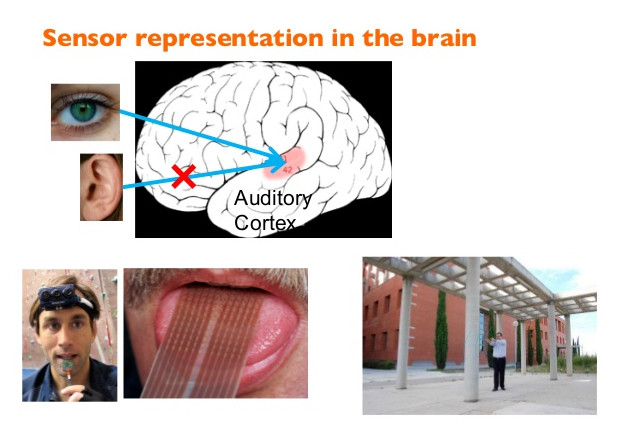
\includegraphics[width=5in]{Figures/OneLearningAlgoAndreNg.jpg}
	\caption[An Electron]{Représentation des sensations dans le cerveau. [Roe et al. 92]}
	\label{fig:Electron}
\end{figure}


	La même expérience a été reproduite avec succès à plusieurs reprises et avec des configurations différentes (différentes régions du cerveau, des espèces différentes, etc.) qui ont conduit aux mêmes résultats.

	L'apprentissage automatique vise à concevoir ce genre d'algorithme, capable à s'adapter à toutes les situations possibles. L'objectif est de trouver des modèles dans les données utilisées pour l'apprentissage, et les généraliser pour construire des modèles mathématiques capables de faire des prédictions pour de nouvelles données.

\section{Concepts de base de l'apprentissage automatique}

	D'après la définition de [Mit et al. 97] "Un programme informatique apprend d'une expérience \textit{E} à effectuer une tâche \textit{T} si sa performance \textit{P} mesurée pour cette tâche \textit{T} s'améliore avec l’expérience \textit{E}."

	La description des notions d'expérience, tâche et performance comme donnée dans le livre [Goo et al. 16] est très claire et peut être vue comme suit :

\subsection{Les tâches \textit{T}} 
	L'apprentissage automatique intervient dans des tâches où l'algorithmique classique est incapable de donner des résultats satisfaisants, ou prendrait simplement trop de temps. Ces tâches peuvent être par exemple des tâches de:\\

\textbf{Classification:} Où le programme doit trouver la classe $c \in C$ à laquelle une entrée \textit{X} appartient. En d'autres termes, on cherche à apprendre une fonction $F : \mathbb{R}^{n} \rightarrow C$ (C étant un ensemble discret ${1..k}$).\\

\textbf{Classification avec manque de données:} Elle rajoute un niveau de difficulté à la tâche de classification en supposant que certaines données peuvent être manquantes. Le classifieur devrait dans ce cas apprendre plusieurs fonctions avec différents sous ensembles des attributs de l'entrée \textit{X}.\\

\textbf{Régression:} Cette tâche ressemble à une classification, sauf que le résultat qui était la classe devient une valeur numérique, et l'espace de sortie devient continu. Nous cherchons donc à trouver une fonction $F : \mathbb{R}^{n} \rightarrow \mathbb{R}$.\\

\textbf{Transcription:} Elle ressemble encore à la classification, sauf que ce que nous cherchons en sortie au lieu d’être une classe, est une séquence de symboles. Comme par exemple, la traduction d'une phrase dans une autre langue.\\

\textbf{Détection d'anomalie:} Où le programme examine constamment une série d’événements ou de données d'entrée et signale s'il trouve quelque chose d'inhabituel. Une de ses applications est la détection de fraude dans l'utilisation de cartes de crédit.\\

\textbf{Dé-bruitage:} Permet d'apprendre à "nettoyer" une entrée \textit{X'} qui pourrait être corrompue par un certain processus de corruption, en retournant l'entrée originale \textit{X}.\\

\subsection{Les mesures de performance \textit{P}}

	La mesure de performance sert d'outil pour déterminer si un programme effectue bien la tâche \textit{T} souhaitée. Elle diffère d'une tâche à une autre.
	
	La mesure se fait sur les données dont on dispose et qu'on utilise pour l'apprentissage, mais aussi sur une partie de données mises de côté (non utilisées pour l'apprentissage). Le plus important étant de savoir si le programme retourne de bons résultats sur des instances qu'il n'a jamais rencontrées.   

	Plusieurs mesures de performance existent pour les tâches de classification, la mesure de précision étant généralement la plus utilisée. Mais pour d'autres tâches, le choix de la mesure peut être plus difficile à faire.

\subsection{L’expérience \textit{E}}

	L'expérience peut être définie par un scénario que le programme est sensé suivre durant son apprentissage, ce scénario est appelé un algorithme d'apprentissage classé en trois grandes catégories:\\
	
\textbf{Non-supervisé:} Le programme reçoit un ensemble de données (des exemples) qu'il se doit d'étudier pour satisfaire une tâche précise qui revient soit à minimiser un coût (pour augmenter la performance), soit à trouver des caractéristiques qui lient les attributs des exemples entre eux, afin de trouver une manière de regrouper ces derniers en catégories. Par exemple: clustering, PCA, etc.\\

\textbf{Supervisé:} Le résultat du traitement de chaque exemple est connu à l'avance. À chaque fois que le programme retourne une valeur de la fonction à apprendre, il compare cette dernière avec la valeur juste (connue), si elle est conforme le programme est sur la bonne voie, sinon des modifications sur la fonction apprise (paramètres appris) doivent être effectuées. Par exemple: Les réseaux de neurones, SVM, arbre de décision, etc.\\

\textbf{Apprentissage par renforcement:} c'est un type différent des deux premiers dans le sens où le programme est perçu comme un agent qui interagit dans un environnement, et qui reçoit des feedbacks (réponses ou retours d'information) lui permettant d’établir une "politique" qui vise à maximiser ses "gains" ou "récompenses". Par exemple: Q-learning.\\


\subsection{Exemple d'algorithme d'apprentissage: Les réseaux de neurones}
	
	Nous allons maintenant présenter l'une des techniques les plus utilisées pour l'apprentissage automatique supervisé (et aussi pour le non-supervisé), à savoir les réseaux de neurones (Perceptron Multicouche).
	
	Un réseau de neurones artificiel essaye d'imiter le fonctionnement des réseaux de neurones biologiques. Appelé aussi perceptron multicouche, ces derniers sont comme leur nom l'indique, formés de plusieurs couches de neurones, la première est la couche d'entrée, ensuite viennent celles du milieu qui sont les couches cachées et à la fin une dernière couche appelée couche de sortie. La figure [Figure 2.2] ci-dessous montre un exemple d'un réseau de neurones à une seule couche cachée:


\begin{figure}[H]
	\centering
		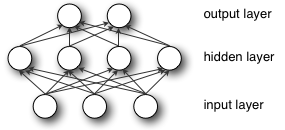
\includegraphics[width=3in]{Figures/mlp.png}
	\caption[An Electron]{Réseau de neurones (FC-MLP) à une seule couche cachée.}
	\label{fig:Electron}
\end{figure}

	Un réseau de neurones fonctionne comme suit: La couche d'entrée reçoit d'abord une combinaison de valeurs qu'elle va transmettre à tous les neurones, de la couche cachée, qui la suivent. Chaque neurone de la couche cachée reçoit en entrée une combinaison linéaire d'entrées (vecteur de valeurs), la multiplie par le poids \textit{w} du neurone, et y rajoute un biais \textit{b}. Le résultat sera ensuite envoyé à une fonction d'activation \textit{s} qui peut être par exemple la fonction $Sigmoide(x) = 1/(1+e^{x})$.
	
	Une fonction d'activation de la couche de sortie \textit{G} est choisie, cette dernière est choisie selon la tâche voulue (par exemple: régression, classification, etc.).
Tout le processus est schématisé par un calcul matriciel. L’expression de la fonction \textit{f} que le réseau de neurones essaye d'apprendre est comme suit:

$$f(x) = G( b^{(2)} + W^{(2)}\times( s( b^{(1)} + W^{(1)}\times x)))$$

	Avec \textit{x} vecteur d'entrée et \textit{w1}, \textit{ b1}, \textit{w2} et \textit{b2} étant les matrices de poids et vecteur biais entre respectivement la couche d'entrée et la couche cachée, et entre la couche cachée et la couche de sortie. Ce sont ces paramètres qui seront appris.
	
	Nous allons ensuite réaliser un apprentissage du réseau de neurones et donc essayer de se rapprocher de la fonction qu'on souhaite apprendre. Les paramètres à apprendre (\textit{w1}, \textit{ w2}, \textit{b1} et \textit{b2}) seront changés à chaque itération grâce à différents algorithmes, le plus utilisé étant l'algorithme rétro-propagation du gradient (backpropagation of errors). 
	Ayant le résultat souhaité (réel) et le résultat retourné, l'idée est de définir une fonction "coût" (l'inverse de la performance) qui décrira à quel point la fonction \textit{f} est éloignée de ce qui est recherché. Ensuite dériver \textit{f} en fonction de chacun de ses paramètres, et changer ces derniers dans le sens qu'il faut (rajouter à sa valeur, ou en soustraire), dans le but de faire diminuer la valeur du coût.

	Comme mentionné précédemment, l'apprentissage d'une tâche \textit{T} est sensé permettre une application de ce qui a été acquis sur de nouvelles données, ceci est appelé la capacité de généralisation. La généralisation d'un apprentissage peut faire face à plusieurs problèmes [figure 2.3], les plus importants sont:\\

\textbf{Le sur-apprentissage:} Quand le programme retourne de bons résultats sur les données d'apprentissage, mais n'arrive pas à généraliser sur des données qu'il n'a jamais rencontrées auparavant.\\

\textbf{Le sous-apprentissage :} Dans le cas où le programme n'arrive même pas à trouver un modèle qui satisfait les données de l'apprentissage.\\


\begin{figure}[H]
	\centering
		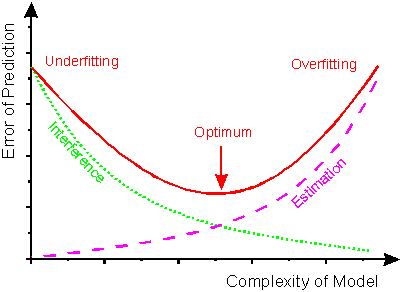
\includegraphics[width=3in]{Figures/image024.png}
	\caption[An Electron]{Sur-apprentissage et sous-apprentissage. [Mar et al. 89]}
	\label{fig:Electron}
\end{figure}


\section{Introduction à l'apprentissage profond}

	Comme nous l'avons mentionné, l'une des techniques les plus récentes en apprentissage automatique est l'apprentissage profond, elle est composée de deux mots: apprentissage et profond. La première partie se réfère au fait que ce soit un concept d'apprentissage automatique, et la deuxième partie: profond, se réfère à sa structure.

	Principalement en raison de la faible puissance de calcul des machines, les algorithmes d'apprentissage n'étaient pas très complexes et puissants. Mais grâce à l'évolution exponentielle de la puissance de traitement (loi de Moore [Moo 65]) de nouvelles perspectives ont été mises en lumière.
Depuis 2010, l'utilisation de la puissance des GPUs pour les calculs est devenue accessible pour le grand public, les scientifiques sont en mesure d'effectuer efficacement des calculs parallèles sur de très grosses matrices, et donc, ils ont réussi à élargir leurs modèles d'algorithme d'apprentissage pour atteindre de manière significative de meilleurs résultats et performances.

	L'apprentissage profond permet de développer des approches d'apprentissage automatique de plus en plus profondes (plus volumineuses et donc plus complexes), mais il permet aussi une très grande flexibilité qui lui permet de combiner plusieurs techniques différentes. Pourtant, beaucoup de problèmes restent à régler, un des plus gros étant la soi-disant curse of dimentionality (la malédiction de la dimensionnalité). En fait, les données en entrée à un algorithme d'apprentissage sont de haute dimensionnalité. Une image par exemple, est une matrice de milliers, ou peut-être même de millions de pixels, chacun peut prendre des centaines de valeurs différentes (les valeurs RGB). Si nous prenons par exemple une image de $100 \times 100$, le nombre de configurations distinctes qu'elle peut prendre est:
$256^{3} \times 100 \times 100 = 1 677 721 600$.

	Cet espace de valeurs est évidemment trop grand pour pouvoir en couvrir même une fraction. Mais le problème serait plus à propos des fonctions de hautes variations que nous essayons de reproduire (fonctions d'apprentissage). En fait, si la fonction n'est pas trop complexe, même dans des dimensions élevées, quelques exemples pourraient être suffisants pour l'apprentissage de sa représentation, mais si la fonction cible a beaucoup de variations, nous aurons besoin en conséquence de plusieurs exemples d'apprentissage, comme le montre la figure [Figure 2.4] ci-dessous:

\begin{figure}[H]
	\centering
		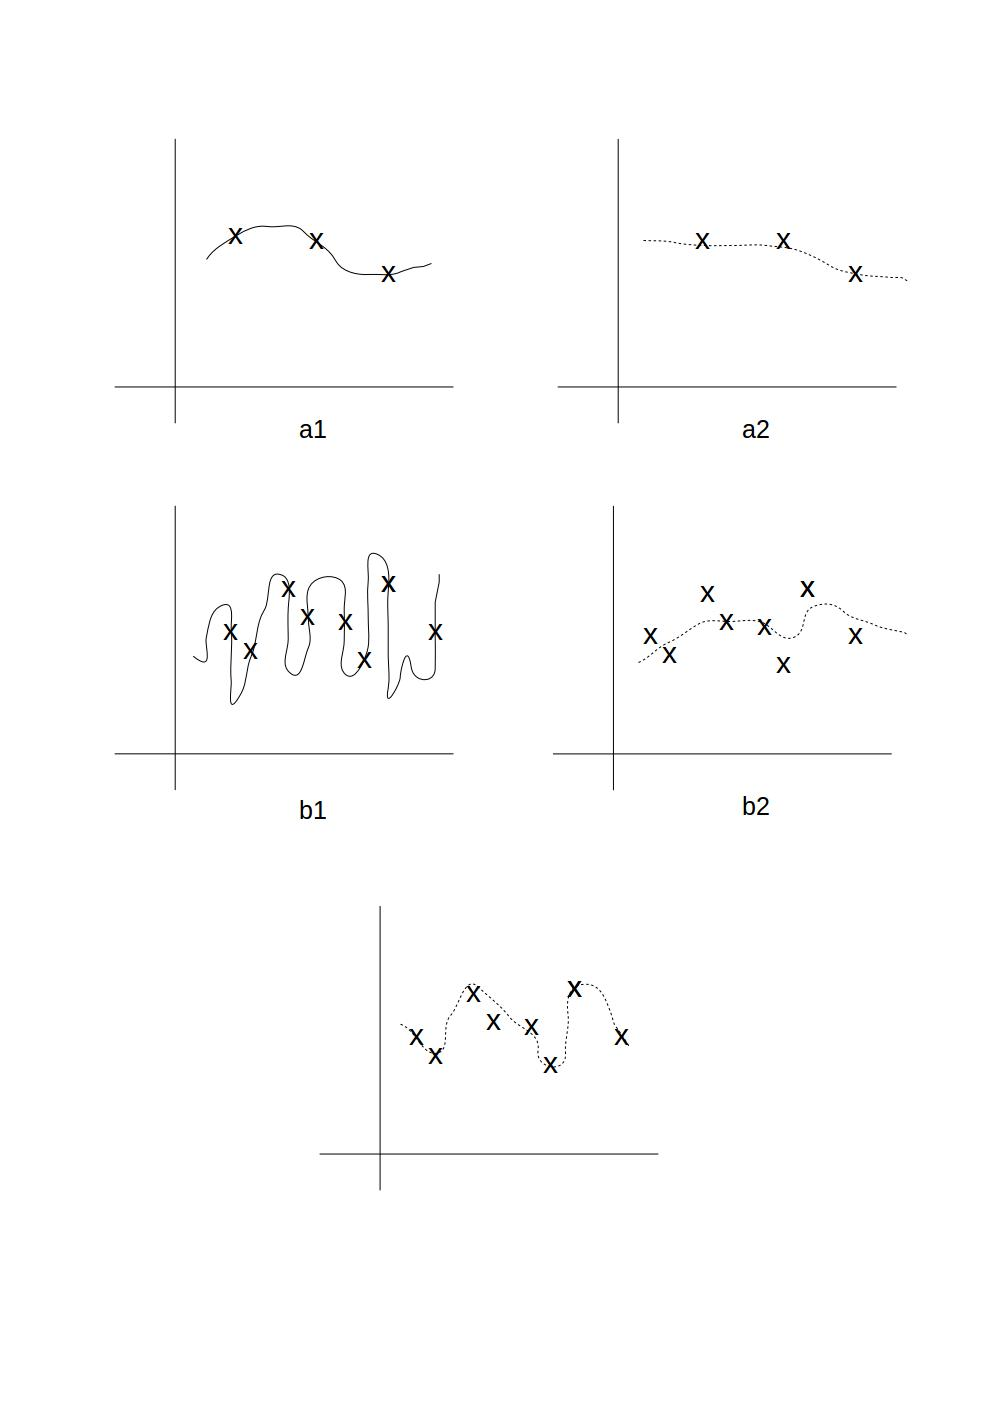
\includegraphics[width=3in]{Figures/highVariation.jpg}
	\caption[FA]{Fonctions d'approximation.}
	\label{fig:Electron}
\end{figure}


	Pour une fonction à deux dimensions (deux attributs), nous avons dans l'exemple (a) le graphe (a1) qui montre une fonction simple que le modèle cherche à approximer, et le graphe (a2) montre le résultat de l'approximation obtenu par le modèle. Ce résultat est satisfaisant malgré le nombre réduit d'exemples.

	Quant à l'exemple (b), le graphe (b1) montre une fonction beaucoup plus complexe que celle du graphe (a1), la tâche d'approximation devient plus difficile. Les tentatives du modèle (représentées respectivement par les graphes (b2) et (b3)) de ne pas passer par tous les exemples, ou de passer par tous les exemples échouent à trouver un résultat satisfaisant dans les deux cas. On vise à trouver une approximation de la fonction qui passe par tous les exemples, et donc si on trouve une fonction qui passe par tous les exemples mais qui ne ressemble pas à la fonction qu'on veut approximer, on fera face à un problème de sur-apprentissage.

	Il est clair que pour une dimension \textit{D} plus grande de donnée en entrée (exemple: age, salaire, etc.) ou sur une variété de dimension D, le nombre de variations peut croître de façon exponentielle avec \textit{D}, d'où résulte le grand nombre d'exemples requis. [Ben 14]

\section{Les architectures de l'apprentissage profond}

	Bien que le principe des algorithmes d'apprentissage existants est unique (en consistant à passer par un tas de données pour trouver des modèles significatifs, et arriver à construire des modèles mathématiques afin de réaliser une tâche d'apprentissage, permettant de s'adapter à des objectifs différents). Plusieurs concepts et architectures sont appliqués pour l'apprentissage profond, parmi eux:

\subsection{Deep Belief Networks}

	Réseaux profond de croyance (DBN) est une pile de machines de Boltzmann restreintes (Restricted Boltzmann Machines RBM) qui se termine généralement avec une unité de classification. Un RBM est un réseau de neurones à deux-couches (une visible et l'autre cachée) stochastique (l'activation de neurones est probabiliste).
Les réseaux profonds de croyance sont utilisés pour le pré-apprentissage non-supervisé, dans le but d'obtenir une meilleure initialisation des poids du réseau.


\subsection{Réseau de neurones à convolution}
	
	L'idée a été inspirée du travail de Hubel et Wesley sur le cortex visuel du chat [Hub et al. 68]. Un réseau de neurones à convolution ou Convolutional Neural Network (ConvNets), vise à émuler le réseau de neurones biologiques.
	La mise en œuvre la plus commune d'un réseau de neurones à convolutions se retrouve dans le réseau LeNet de [Lec et al. 98], il empile différentes couches de piles de convolution et de sous-échantillonnage, suivies à la fin de perceptrons multicouches entièrement connectées, comme indiqué sur la figure suivante :

\begin{figure}[H]
	\centering
		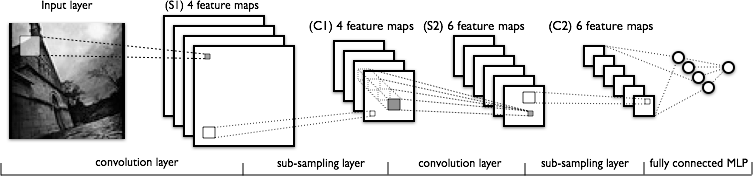
\includegraphics[width=5in]{Figures/Mylenet.png}
	\caption[An Electron]{Réseau à convolution LeNet. [Lec et al. 98]}
	\label{fig:Electron}
\end{figure}

	Nous allons maintenant décrire des notions de bases qui peuvent être utilisées dans les couches d'un réseau de neurones à convolution, telles que le padding, sous-échantillonnage (pooling), normalisation et dropout.

\subsubsection{La convolution}
	
	La convolution est un terme mathématique, elle est définie comme l'application d'une fonction de façon répétée à travers la sortie d'une autre fonction. Dans ce contexte, on applique un filtre sur une image en prenant en compte tous les décalages possibles. Comme le montre la figure suivante:


\begin{figure}[H]
	\centering
		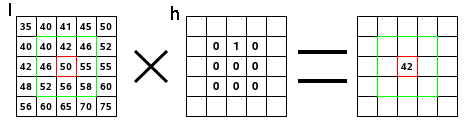
\includegraphics[width=5in]{Figures/convExample.png}
	\caption[An Electron]{Exemple de convolution.}
	\label{fig:Electron}
\end{figure}

	Soit une image \textit{I} et un filtre de convolution \textit{h}, appliquer un filtre de convolution sur un pixel, par exemple le pixel au centre avec la valeur 52, signifie donner une nouvelle valeur (égale à 42) à ce pixel en appliquant le filtre sur ce pixel et ses voisins, comme le montre la figure [Figure 2.6].
	
	Les couches de piles de convolution appliquent simplement une multitude de convolutions sur les couches du réseau en utilisant différents filtres.

\subsubsection{Le padding}

	L'application d'une convolution ne peut pas se faire sur les pixels des bords de l'image, cela donc réduira la taille de l'image après qu'elle soit filtrée. Afin de pouvoir mieux contrôler la taille des images obtenues après l'application d'une convolution sur une image en entrée, on peut utiliser ce qu'on appelle "padding" (remplissage) avant l'application d'un filtre de convolution.
	L'une des techniques utilisées pour le padding est le zero-padding, pour cela il suffit de rajouter des zéros aux bords de l'image. Pour un zero-padding de 1, on a le résultat de la figure suivante:

\begin{figure}[H]
	\centering
		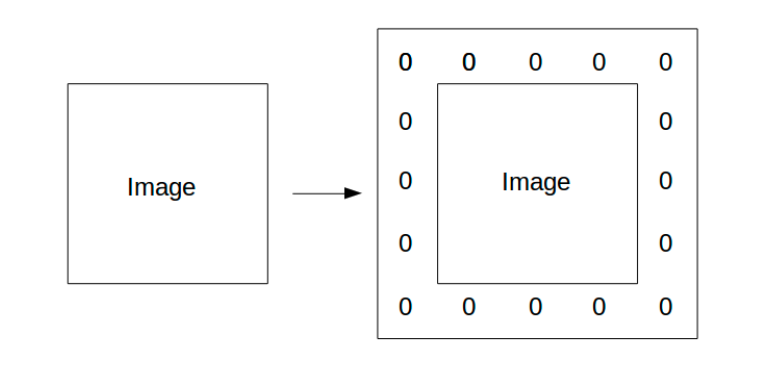
\includegraphics[width=5in]{Figures/zero-padding.png}
	\caption[An Electron]{Application d'un zero-padding sur une image}
	\label{fig:Electron}
\end{figure}

	Nous pouvons aussi utiliser le zero-padding pour conserver exactement la taille spatiale d'une image après l'application d'une convolution, de sorte à ce que la largeur d'entrée et de sortie et la longueur restent les mêmes, comme nous le verrons dans le prochain chapitre. [CS231n 16]


\subsubsection{Le sous-échantillonnage}

	Le sous-échantillonnage (subsampling) se réfère à la réduction de la taille globale d'un signal. Applicable dans de nombreux cas, comme la compression audio pour les fichiers de musique, le sous-échantillonnage se fait simplement pour réaliser une réduction de la taille des données. 

	La méthode de sous-échantillonnage spécifique proposé par LeCun dans LeNet est connue comme max-pooling. Cela implique le fractionnement d'une matrice (image) en de petits fragments qui ne se chevauchent pas (plus les fragments sont grands, plus la réduction est importante), et de prendre la valeur maximale dans chaque grille en tant que valeur dans la matrice réduite. 
	Ceci permet, entre autres, l'obtention d'une invariance aux translations. La figure suivante montre un exemple de l'application d'un max-pooling:

\begin{figure}[H]
	\centering
		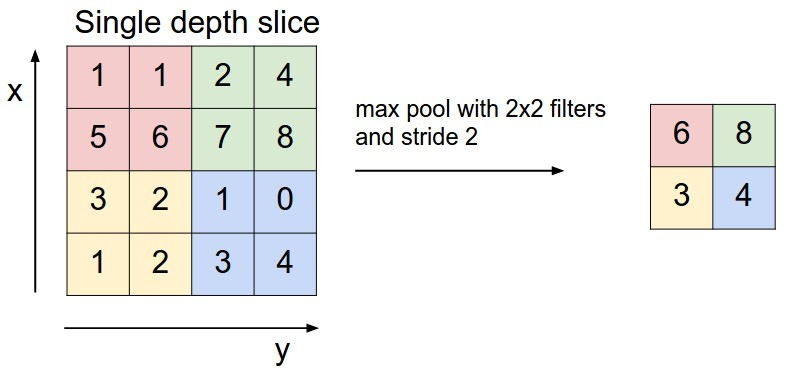
\includegraphics[width=5in]{Figures/maxpool.jpeg}
	\caption[MP]{Exemple de max-pooling.}
	\label{fig:Electron}
\end{figure}


\subsubsection{Normalisation}

	Une des techniques utilisée, inspirée de la neuroscience computationnelle, est l'ajout de couches de normalisation après une couche de convolution [Kri et al.,12]. Néanmoins, l'application d'une normalisation sur ces couches semble avoir un impact très minime et n'est plus utilisée. Ils ont été dominés par d'autres techniques telles que le "dropout" ainsi qu'une meilleure initialisation des poids des neurones et les algorithmes d'entraînement du réseau. [CS231n 16]
	
\subsubsection{Perceptron multicouche entièrement connecté}

	A la fin du réseau, après plusieurs couches de mise en commun de convolution et de max-pooling, le traitement final dans le ConvNets se fait via des couches de perceptrons entièrement connectés. Une couche entièrement connectée prend tous les neurones de la couche précédente et les relie à chaque neurone dont elle dispose.

\subsubsection{Dropout}

	On applique un dropout lors de la phase d'entraînement d'un réseau de perceptron multicouche entièrement connecté (FC-MLP), précisément lors de la rétro-propagation. Son but est d'éviter le sur-apprentissage, par exemple pour un taux de dropout de 30\%, la rétro-propagation ne s'appliquera pas sur 30\% des neurones d'une couche (ces neurones sont choisis aléatoirement à chaque rétro-propagation). Dans ce cas les neurones d'une même couche n'auront pas rencontré (n'apprendront pas) les même exemples (images). Cela procurera au réseau une plus grande capacité de généralisation.

\subsection{Deep AutoEncoders}

	Les Autoencoders sont l'un des concepts introduits par l'apprentissage profond. Nous avons déjà parlé du problème de curse of dimentionality, les autoencoders proposent un moyen de résoudre ce problème. Pour cela, ils visent à trouver une représentation compressée des données en entrée.
	
	En d'autres termes, les autoencoders sont un type de réseaux de neurones entraînés d'une manière supervisée par rétro-propagation pour reproduire leurs données en entrée après les avoir fait passer à travers des couches cachées de dimension inférieure à celle de l'entrée, nous donnerons plus de détails sur le fonctionnement d'un autoencoder dans le prochain chapitre.

%Une des techniques pour former un "deep autoencoder" de empilant pré-entraîné, et d'ensuite faire une mise au point à la fin avec de la rétropropagation.

	Un "deep autoencoder" est construit en empilant un certain nombre de couches de machines de Boltzmann restreintes RBM pré-entraînées (formant un réseau profond de croyance DBN). On applique à la fin sur ces couches un ajustement ou une mise au point (fine tuning) avec de la rétro-propagation (backprop). La figure suivante montre un exemple d'autoencoder:

\begin{figure}[H]
\centering
	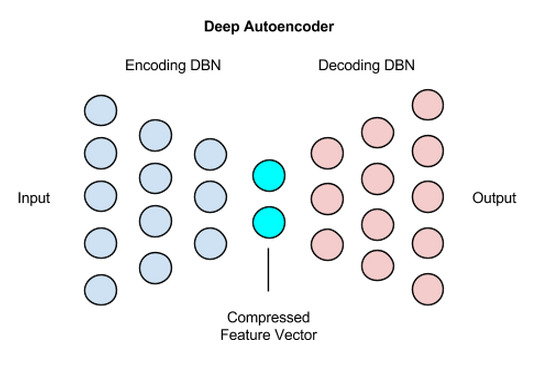
\includegraphics[width=3in]{Figures/deep_autoencoder.png}
\caption[An Electron]{Exemple d'un modèle d'autoencoder utilisant les DBN.[Site1]}
\label{fig:Electron}
\end{figure}

	Un exemple d'utilisation d'un autoencoder est la recherche d'une représentation de dimension inférieure pour une image. La raison pour laquelle cette représentation pourrait exister est donnée par l'idée suivante: Si vous essayez de générer une image aléatoire, vous vous retrouverez très probablement avec une image comme le montre la figure suivante:

\begin{figure}[H]
	\centering
		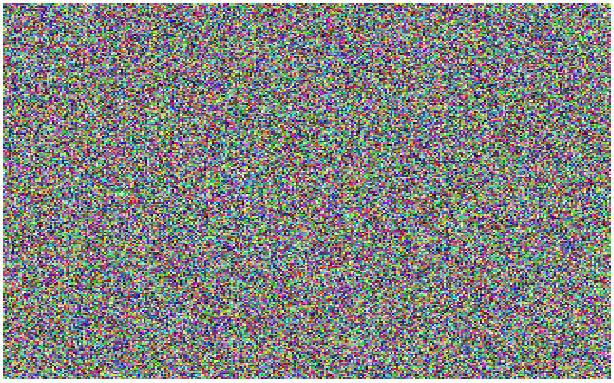
\includegraphics[width=3in]{Figures/randomImageGEn.JPG}
	\caption[An Electron]{Image générée aléatoirement.}
	\label{fig:Electron}
\end{figure}

	Peu importe combien de fois vous essayerez, vous n'obtiendrez probablement jamais une image d'un chien, d'une voiture, ou une autre chose significative.
Ainsi, l'espace des images significatives forme seulement une fraction de l'espace total défini par les valeurs des pixels. L'objectif de l'autoencoder est alors de trouver une représentation significative d'une image dans cet espace.

\section{Les exploits des techniques d'apprentissage profond [Site2]}

	L'Apprentissage profond a surperformé les techniques de vision artificielle traditionnelles au cours des dernières années. Dans le concours ImageNet en 2010 (ImageNet est un projet qui a pour but de fournir aux chercheurs une très grande base d'images facilement accessible), le meilleur algorithme de vision artificielle traditionnelle avait obtenu un taux d'erreur de 28,2\%, ce qui signifie qu'il a obtenu de 71.8\% d'images correctes. En 2011, le meilleur algorithme a obtenu un taux d'erreur de 25,8\%. 

	En 2012, cependant, le premier processus d'apprentissage profond est entré dans la compétition et a dépassé en performance toutes les méthodes traditionnelles, en obtenant un taux d'erreur de 16,4\%.
	Après cela, le premier algorithme d'apprentissage profond a ouvert les portes, la compétition a été inondée avec d'autres équipes d'apprentissage profond qui ont atteint un taux d'erreur de 11,7\% en 2013 et 7.405\% en 2014. Le vainqueur de l'édition 2014 a reconnu presque 93\% des images, un énorme bond en avant surtout par rapport au taux de 72\% atteint par les techniques de vision artificielle traditionnelles en 2010. La figure suivante montre les résultats des dernières années du concours d'ImageNet:

\begin{figure}[H]
	\centering
		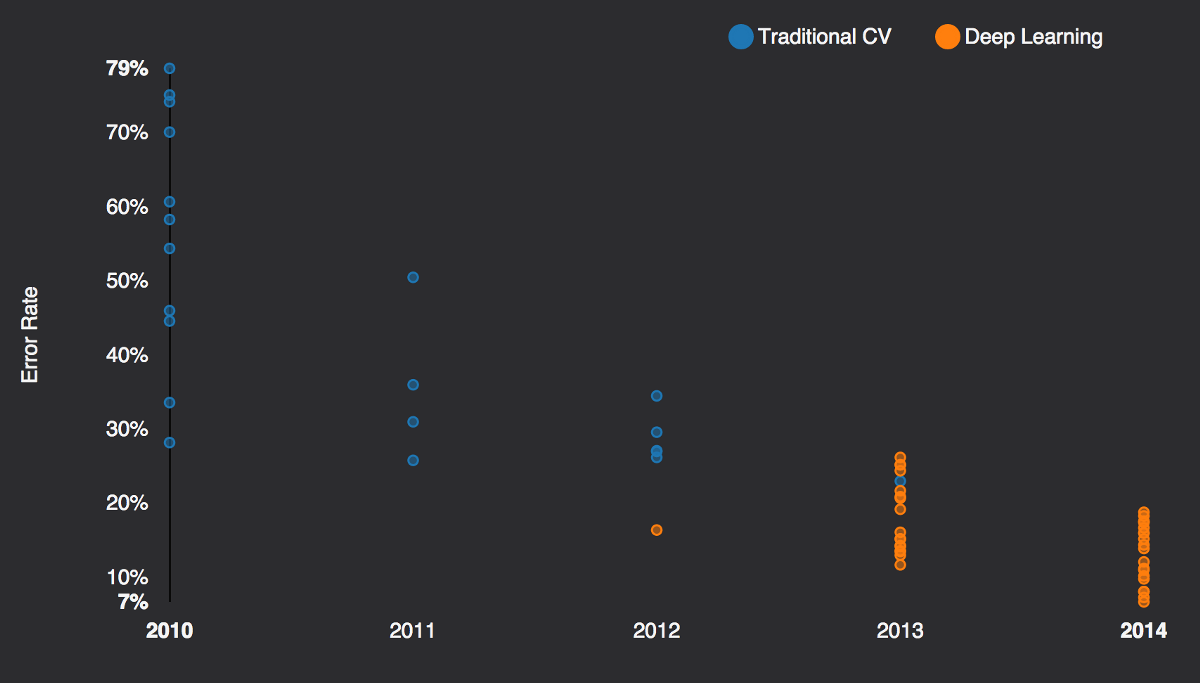
\includegraphics[width=5in]{Figures/clairifaiIMAGENET.png}
	\caption[An Electron]{Résultats du concours d'ImageNet. [Site2]}
	\label{fig:Electron}
\end{figure}

	En voyant ces résultats phénoménaux, beaucoup de laboratoires ce sont convertis vers ces approches et y consacrés une grande partie de leurs efforts. On peut citer les laboratoires de grandes université tel que: l'université de Berkeley, Stanford, Bonn, Berlin, Oxford, Montréal, Toronto. Mais aussi des laboratoires de grande entreprises tel que: Facebook AI Research, Google Research, Twitter’s Deep Learning Group, Microsoft Research.\\

	L’Intérêt croissant des entreprises au domaine de l'apprentissage profond fait naître des initiatives et des prototypes pour des produits plus intéressants les uns que les autres, et pousse donc la recherche. Parmi ces produit on peut noter les véhicules autonomes avec \textbf{Google Self-Driving Car}, mais aussi le lancement du \textbf{Tesla Autopilot} sur les nouvelles voitures Tesla depuis déjà quelques mois. Et enfin les testes en échelle réelle d'un convois d'une douzaine de grands camions auto-pilotés des grands constructeurs Volvo, Daimler, Iveco, MAN, DAF et Scania. Le convoi a parcouru 2000km à travers l’Europe et fut un grand succès. La figure suivante montre quelque exemple des Self-Driving cars:

\begin{figure}[H]
	\centering
		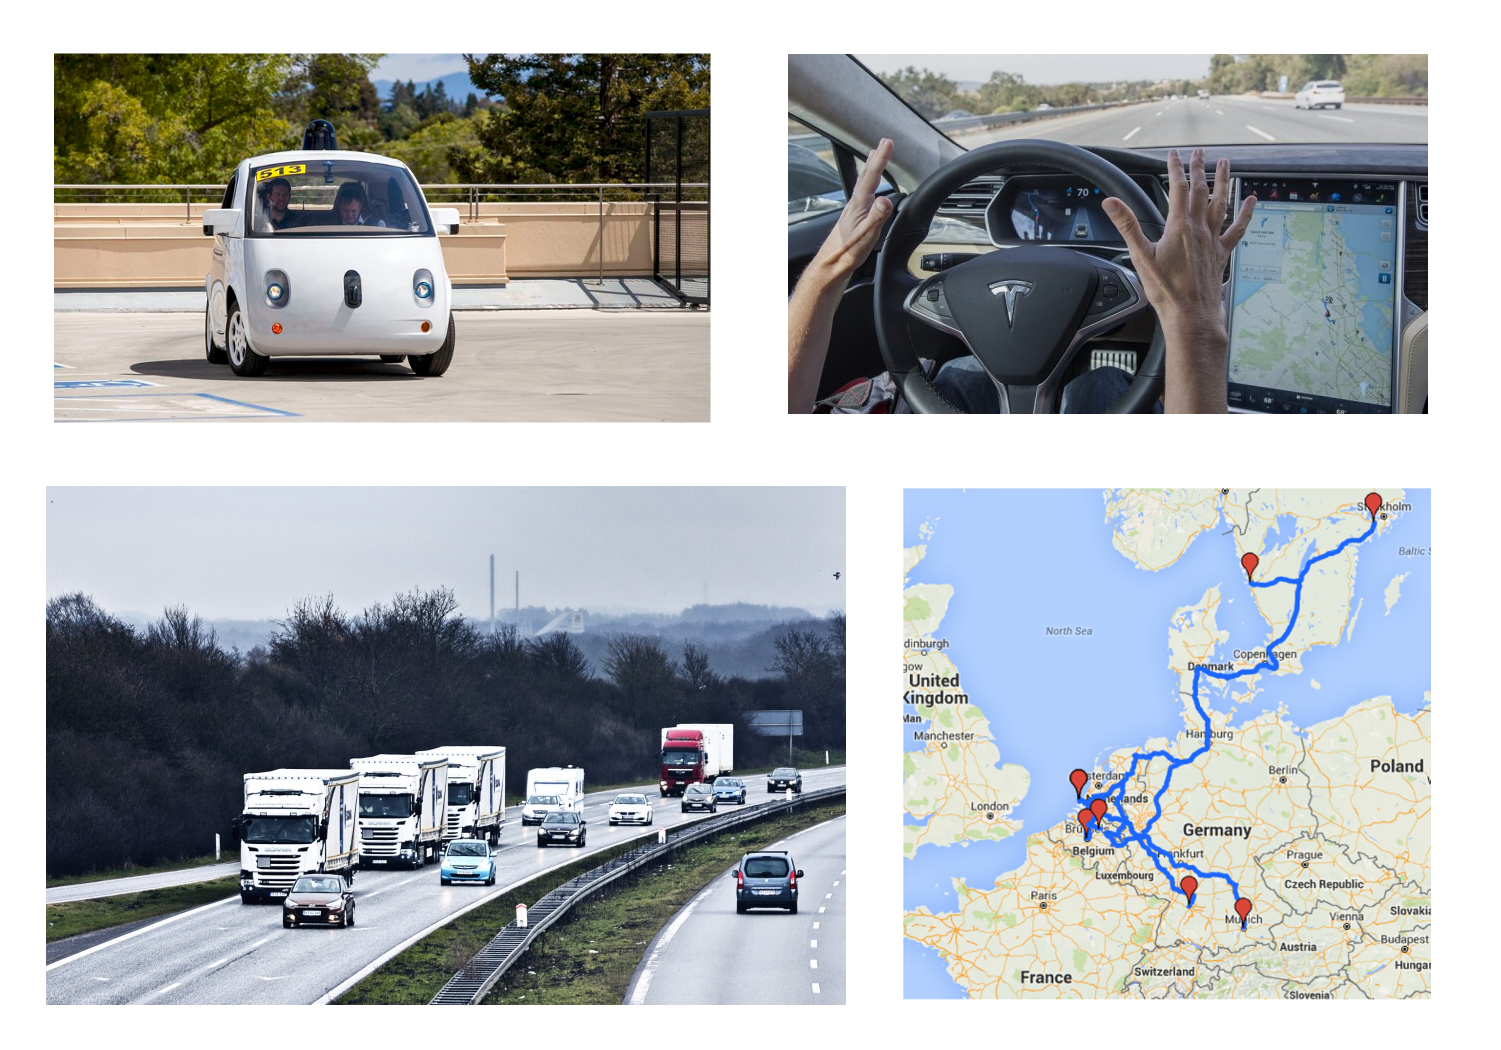
\includegraphics[width=5in]{Figures/selfDriving.png}
	\caption[An Electron]{Respectivement de gauche à droite, et de haut en bas: Google Self-Driving Car; Tesla Autopilot; Le convoi des camions auto-pilotés; le parcours des camions à travers l'Europe.}
	\label{fig:Electron}
\end{figure}


\section{Conclusion}

	Nous avons présenté dans ce chapitre la notion d'apprentissage automatique et sur quelle théorie elle se base, et comme exemple nous avons décrit les réseaux de neurones. L'apprentissage profond est l'une des techniques d'apprentissage automatique les plus récentes, nous avons ensuite fait une introduction sur les différents concepts d'apprentissage profond les plus utilisés.
	
	Nous nous intéresserons dans le prochain chapitre à notre implémentation d'un système de recherche d'images par le contenu en utilisant des concepts d'apprentissage profond, qui sont les réseaux à convolutions et les Deep Autoencoders. Nous effectuerons des mesures de performances pour comparer toutes nos approches, et nous donnerons à chaque fois nos interprétations des résultats obtenus.

